\documentclass[justified, nobib]{tufte-handout}

\usepackage{Haust2017almennt}

\title{Tölvunarfræði 1a  \semester - Námsáætlun og upplýsingar}

\begin{document}

\section{Námsáætlun}
\label{sec:schedule}

Námskeiðið er grundvallarnámskeið í tölvunarfræði og forritun, sérstaklega ætlað nemendum í vísindum og verkfræði.

\begin{marginfigure}
\caption{Merki Matlab}
\begin{center}

\includegraphics[width=0.5\linewidth]{matlab-logo}
\end{center}
\end{marginfigure}

Forritunarmálið sem notað verður í námskeiðinu er Matlab. Forritunarmálið og aðferðir sem því tengjast henta vel til vísindalegra útreikninga og gagnavinnslu.

\begin{table*}
\caption{Námsáætlun eftir vikum}
\label{tab:schedule}
\begin{center}
\renewcommand{\arraystretch}{1.2}
\begin{tabularx}{\linewidth}{lccXp{3cm}}
\toprule
&\multicolumn{2}{c}{Dagsetningar}&&\\
\cmidrule{2-3}
Vika&Þri&Fös&Námsefni&Kaflar\\
\midrule
1	&22/8	&25/8	& Kynning, Matlab-uppsetning, bitar og tvíundartölur, breytur, innbyggð föll, slembitölur &1.1 til 1.6\\
2	&29/8	&1/9	& Vigrar og fylki&2.1 til 2.5\\
3	&5/9	&8/9	& Reiknirit, skipanaskrár, inntak og úttak, einfaldar myndir&3.1 til 3.6\\
4	&12/9	&5/9	& Notendaskilgreind föll, stýrisetningar, röksegðir, \texttt{is}-föll&3.7, 4.1 til 4.6\\
5	&19/9	&-	    & For-lykkjur&5.1 til 5.2\\
6	&26/9	&29/9	& While-lykkjur, frekari vigurvinnsla, skipulag forrita, gildissvið breyta, kommutölur&5.3 til 5.5, 6.1, 6.2\\
7	&3/10	&6/10	& Gildissvið breyta, aflúsun. Strengir, aðgerðir á strengi&6.4, 6.5, 7.1 til 7.2\\
\cmidrule{4-4}
\multicolumn{5}{c}{Miðmisserispróf á laugardegi}\\
\cmidrule{4-4}
8	&10/10	&13/10	& Föll fyrir strengi, umbreytingar milli strengja og talna, hólfavigrar&7.3, 7.3, 8.1\\
9	&17/10	&20/10	& Færslur, skráarvinnsla&8.1, 9.1\\
10	&24/10	&27/10	& Frekari skráarvinnsla, MS Excel skrár, MAT-skrár&9.1 til 9.3\\
11	&31/10	&3/11	& Nafnlaus föll, fallshandföng, breytilegur fjöldi stika, hreiðruð föll, endurkvæm föll&10.1 til 10.5\\
12	&7/11	&10/11	& Öflugri teikniskipanir, hreyfimyndir, þrívíðar teikningar, teiknihandföng&11.1 til 11.7\\
13	&14/11	&17/11	& Tölfræðiföll, mengjaaðgerðir, röðun, helmingunarleit&12.1 til 12.3, 12.5\\
14	&21/11	&24/11	& Myndvinnsla, mátun ferils, samantekt&14.1\\
\bottomrule
\end{tabularx}
\end{center}
\end{table*}

\section{Kennari}
Aðalkennari er Eiríkur Ernir Þorsteinsson. Aðsetur er í Tæknigarði, 2. hæð, stofa 214. Sjá mynd \ref{fig:taeknigardur}.

\begin{marginfigure}
    \caption{Önnur hæð í Tæknigarði}
    \label{fig:taeknigardur}
    \begin{center}
    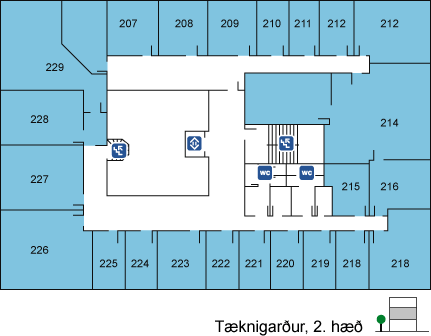
\includegraphics[width=\linewidth]{taeknigardur}
    \end{center}
\end{marginfigure}

Til að hafa samband við kennara er ráðlagt að setja inn þráð á \href{piazza.com/hi.is/fall2017/tl105g/home}{Piazza}. Allar fyrirspurnir sem ekki fela í sér persónulegar upplýsingar ættu að fara þangað. Tölvupóstfang er \href{mailto:ernir@hi.is}{ernir@hi.is}.

Ef um veikindi, námsörðugleika eða áföll er að ræða skal hafa samband við Náms- og starfsráðgjöf HÍ, sjá \nameref{sec:help} hér að neðan.

\section{Tímar og námstilhögun}
Aðalkennsla fer fram í vikulegum fyrirlestrum. Fyrirlestrarnir eru á þriðjudögum klukkan 10 í HT-102 og föstudögum klukkan 12:30 í VRII-157.

Dæmatímar eru á mánudögum og þriðjudögum. Nemendum er frjálst að mæta í þá dæmatíma sem henta best.\footnote{Kennari mun skerast í leikinn ef sókn í dæmahópana verður mjög ójöfn.}

\subsection{Mætingaskylda}
Ekki er skylda að mæta í fyrirlestra eða dæmatíma (en sjá \nameref{sec:lecture-exercises}). Nemendur eru ábyrgir fyrir því að forgangsraða tíma sínum.
\subsection{Upptökur á fyrirlestrum}
Fyrirlestrar eru teknir upp þegar tæknin leyfir. Varað er við því að treysta á upptökur í stað mætingar í fyrirlestra þar sem upptökur geta brugðist og upplifunin er ekki sú sama.

Um verður að ræða upptökur af skjá kennara ásamt hljóði.
\subsection{Álag}
Námskeiðið er $6 ECTS$ einingar. 60 ECTS einingar eru skilgreindar sem 1500-1800 klst. af vinnu.
\[
\text{60 ECTS = 1650 klst.} \Longleftrightarrow \text{6 ECTS = 165 klst.}
\]
Misserið er 14 vikur, svo gera má ráð fyrir 11-12 klst. af vinnu í hverri viku. Þar af eru 4 klst. í fyrirlestrum og dæmatímum.
\section{Bók}
\begin{marginfigure}
    \caption{Kennslubók}
    \begin{center}
    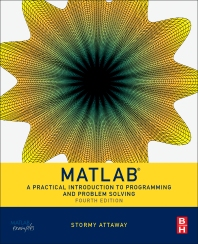
\includegraphics[width=0.8\linewidth]{matlab_stormy_v4}
    \end{center}
\end{marginfigure}
Kennslubók er \emph{Matlab, Fourth Edition: A Practical Introduction to Programming and Problem Solving}, fjórða útgáfa, eftir Attaway.

Eldri útgáfur bókarinnar ættu að mestu leyti að vera gjaldgengar.

\section{Námsmat, einkunnir og próf}
Heildareinkunn er samsett úr prófseinkunn og vetrareinkunn.

\newthought{Vetrareinkunn er 40\% af lokaeinkunn}. Hún er samsett úr einkunn fyrir fyrirlestraræfingar og einkunn fyrir skilaverkefni. Sé einkunn fyrir fyrirlestraræfingar hærri en einkunn fyrir skilaverkefni gilda fyrirlestraræfingar 10\% af lokaeinkunn og skilaverkefni 30\%, annars gilda fyrirlestaræfingar 0\% og skilaverkefni 40\%.

\newthought{Prófseinkunn er 60\% af lokaeinkunn}. Hún er samsett úr einkunn fyrir miðmisserispróf og einkunn fyrir lokapróf. Sé einkunn fyrir miðmisserispróf hærri en einkunn fyrir lokapróf gildir miðmisserispróf 20\% af lokaeinkunn og lokapróf 40\%, annars gildir miðmisserispróf 0\% og lokapróf 60\%.
\subsection{Fyrirlestraræfingar}
\label{sec:lecture-exercises}
Fyrirlestraræfingar eru í hverjum fyrirlestri. Þátttaka í $2n$ fyrirlestraræfingum gefur hluteinkunnina $n$, að hámarki 10.

Til að koma á móts við nemendur sem ekki geta mætt í fyrirlestra, þá er einkunn fyrir fyrirlestraræfingar eingöngu til hækkunar á móti skilaverkefnaeinkunn\footnote{sjá um samsetningu lokaeinkunnar, hér að ofan}.
\subsection{Skilaverkefni}
Vikuleg verkefnaskil eru í námskeiðinu, sem fyrst og fremst eru forritunarverkefni. Verkefnunum skal skila á Gradescope.com (sjá \nameref{sec:tools}). Athugið að \textbf{ekki er tekið við skilum eftir að Gradescope lokar}.

Nauðsynlegt er að skila fjórum af fyrstu sex skilaverkefnunum til að öðlast próftökurétt.
\subsection{Próf}
Lokapróf og miðmisserispróf eru í námskeiðinu. Leyfilegt verður að taka með eitt blað af glósum (skrifað á báðar hliðar) í prófin. Stefnt er að því að halda miðmisserispróf laugardaginn 7. október. 

Lágmarkseinkunn er 5. Nauðsynlegt er að ná lágmarkseinkunn á lokaprófi sem og í námskeiðinu sem heild til að standast námskeiðið. 
\section{Kennslutól}
\label{sec:tools}
Mælt er með að nemendur skrái sig inn á eftirfarandi þjónustur sem allra fyrst:
\begin{itemize}
 \item \href{piazza.com/hi.is/fall2017/tl105g/home}{Piazza}\footnote{\url{piazza.com/hi.is/fall2017/tl105g/home}} er fyrirspurnavefurinn sem notaður er í námskeiðinu. Skráningin í námskeiðið á að vera sjálfvirk, en hafi það misfarist á að vera hægt að skrá sig handvirkt. Allar spurningar sem snúa að námskeiðinu ættu að fara inn á Piazza frekar en í tölvupóst.
 \item \href{https://gradescope.com/courses/8909}{Gradescope.com}\footnote{\url{gradescope.com/courses/8909}} er vefkerfið sem notað er til að taka við skilaverkefnum. Nemendur þurfa að skrá sig sjálfir á þennan vef. Aðgangskóði námskeiðsins er \texttt{9P7YGM}. Mikilvægt er að skrá sig á Gradescope með fullu nafni (íslenskir stafir eru leyfilegir) og með því að nota HÍ-netfang. Kerfið tekur við \texttt{.pdf} skrám.
\end{itemize}

\section{Heilræði og aðstoð}
Sem og í öðrum háskólanámskeiðum er virkni í námskeiðinu lykill að velgengni. Þar er helst átt við að mæta og taka þátt í tímum\footnote{Það að horfa á upptöku gerir ekki sama gagn!} og gera dæmin sem sett eru fyrir.

Skilaverkefnin eru sérstaklega mikilvæg. Það að taka sér góðan tíma í að kljást við þau er mikið lykilatriði. Þau eiga ekki að vera kvöð til að ljúka af, fyrir flestum eru það verkefnin sem virkilega fá færnina til að síast inn.
\subsection{Aðstoð}
\label{sec:help}
Mikilvægt er að gera sér grein fyrir því hvenær tími er kominn til að leita sér aðstoðar. Mikill meirihluti nemenda þarf aðstoð af einhverju tagi í hverju námskeiði.

Hægt er að fá flestum spurningum sem tengjast námskeiðinu og verkefnunum svarað á Piazza. Betra er að spyrja fyrr en seinna, áður en of mikill tími fer til spillis. Dæmatímakennarar og aðrir lengra komnir nemendur eru líka alltaf allir af vilja gerðir til að hjálpa.

\href{http://www.hi.is/verkfraedi\_og\_natturuvisindasvid/nemendathjonusta\_von}{Nemendaþjónusta VoN}\footnote{\url{hi.is/verkfraedi_og_natturuvisindasvid/nemendathjonusta_von}} getur aðstoðað við allt sem viðkemur námsferlum, uppbyggingu náms og vali á námskeiðum. Nemendaþjónustan hefur aðsetur í Tæknigarði og er mjög aðgengileg.

Ef þörf er á sérstökum úrræðum eða undanþágum skal hafa samband við \href{http://nshi.hi.is/}{Náms- og starfsráðgjöf HÍ}\footnote{\url{nshi.hi.is}}. Hægt er að leita til hennar með öll persónuleg mál sem snúa að náminu.

\end{document}